% !TeX spellcheck = de_DE

%  ******************************************************************************
%  * @file      tex/Grundlagen                                                  *
%  * @author    Mario Hesse                                                     *
%  * @version   v0.1.1                                                          *
%  * @date      16.10.2019                                                      *
%  ******************************************************************************

\clearpage

\section{Grundlagen}

In diesem Abschnitt sollten alle Themen erläutert werden, die zum Verständnis der Arbeit notwendig sind. Hier werden die theoretischen Grundlagen gelegt, mit denen der/die Leser*in den Rest der Arbeit verstehen kann. Fachbücher \cite{Helmke2016,Metelmann2016} sind in diesem Kapitel die bevorzugte Literatur. 

Gute Bilder helfen komplexe Inhalte leichter zu verstehen und geben einen schnellen ersten Eindruck. Daher sollte man in der gesamten Arbeit möglichst viele aussagekräftige Bilder verwenden. \autoref{pic:EinErstesBild} ist ein Beispiel dafür. Falls es sich bei den verwendeten Bildern nicht um eigene Kreationen handelt, muss immer eine Quelle angegeben werden.

\begin{figure}[htbp]
	\centering
	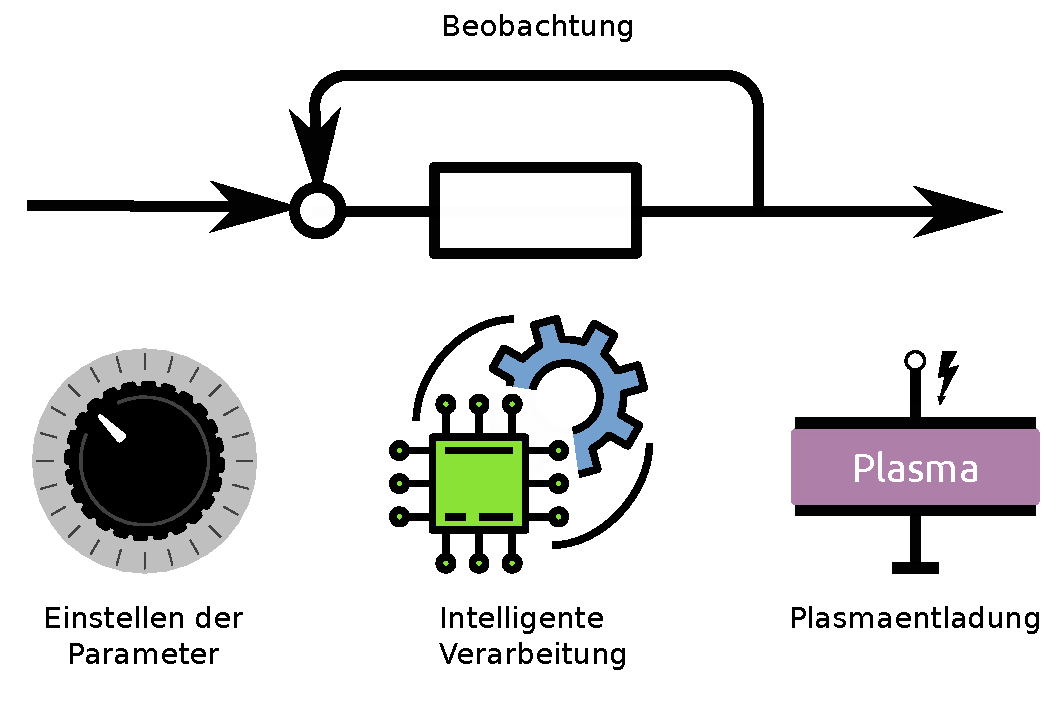
\includegraphics[width=0.5\linewidth]{pic/IntelligentesPlasma.pdf}
	\caption{Ein erstes Bild}
	{\scriptsize Bild: \glqq Intelligentes Plasma\grqq{} von Mario Hesse CC BY 4.0}
	\label{pic:EinErstesBild}
\end{figure}
